% Evans second edition, Chapter 6, printed pp. 293--348 / PDF pp. 310--365.
\chapter[Second-Order Elliptic Equations]{Second-Order Elliptic\\Equations}
\label{chap:second-order-elliptic-equations}
\PDESource
  {Chapter 6; printed pp.~293--348; PDF pages~310--365}
  {中译本：书内第 208--246 页；PDF 第 226--264 页。}

\noindent\textit{Editorial study edition.}
This chapter reconstructs Evans's exposition in original English, with
expanded proofs and Chinese mathematical annotations. It is not a verbatim
transcription. Headings identify the source results; our theorem numbers
run throughout this chapter. All 17 source problems are restated concisely
and solved. Foundational functional analysis is invoked explicitly;
the Schaefer fixed-point theorem and Weyl's asymptotic law are identified
where used or stated, rather than presented as proved here.

\Needspace{45mm}
\PDEAnnotation{弱解到经典解}{存在性先在能量空间中完成，不要求二阶导数。正则性随后补足导数，才能使用经典最大值原理；特征值问题再把紧性与正性结合起来。}
The central example is
\[
 -\operatorname{div}(A Du)+b\cdot Du+cu=f\quad\hbox{in }U,
 \qquad u=0\quad\hbox{on }\partial U.
\]
There are four distinct questions: does a weak solution exist, how smooth
is it, what controls its sign, and when does the homogeneous equation
have a nonzero solution? The answers require different hypotheses.

\paragraph{Conventions and reading route.}
Repeated indices are summed from $1$ to $n$. Unless specified otherwise,
$U$ is a bounded open subset of $\R^n$, $A=(a^{ij})$ is real symmetric,
and $a^{ij}\xi_i\xi_j\geq\theta|\xi|^2$ for some $\theta>0$.
The norm $\|\cdot\|_2$ is over the indicated domain, or over $U$ if omitted.
Begin with \S\ref{sec:6-1}--\S\ref{sec:6-2}, then follow the difference
quotient argument in \S\ref{sec:6-3}. Read \S\ref{sec:6-4} before the
positivity arguments in \S\ref{sec:6-5}. Chapter~5 supplies approximation,
traces, Poincar\'e, difference quotients, and Rellich compactness.
Riesz representation, weak subsequential compactness in Hilbert spaces,
and basic finite-dimensional linear algebra are prerequisites.

\clearpage
% Evans second edition, section 6.1.
% English source: printed p. 293; PDF page 310 (1-based).
% Chinese subsection/page correspondence: pending verification against the scan.
% Status: outline-only; no source text or proof has been transcribed/reviewed.
\section{Definitions}
\label{sec:6-1}

\PDEPending

% TODO: English exposition with source theorem/equation identifiers.
% TODO: Add necessary \PDEVocab, \PDEIdea, or \PDEChinese notes.
% TODO: Expand abbreviated arguments in expandedproof/proofdetails.
% TODO: Verify hypotheses, endpoints, constants, limits, and cross-references.

% Evans 6.2: English printed p.297 / PDF p.314; Chinese printed p.210 / PDF p.228.
\Needspace{65mm}
\section{Existence of Weak Solutions}
\label{sec:6-2}
\subsection{Lax--Milgram (Evans \S6.2.1, Theorem 1)}
\begin{theorem}\label{thm:6-lax-milgram}
Let $H$ be a real Hilbert space. Suppose a bilinear form $B$ satisfies
\[
 |B[u,v]|\leq M\|u\|_H\|v\|_H,\qquad
 B[u,u]\geq\beta\|u\|_H^2,\quad\beta>0.
\]
For each bounded linear functional $\ell$ on $H$ there is a unique $u\in H$
with $B[u,v]=\ell(v)$ for all $v\in H$. Moreover,
$\|u\|_H\leq\beta^{-1}\|\ell\|_{H^*}$.
\end{theorem}
\Needspace{45mm}
\PDEAnnotation{强制性排除失控方向}{有界性保证双线性型连续；强制性则使 $B[u,u]$ 控制整个空间范数。这里不要求 $B$ 对称，所以不能一律把证明改写成能量最小化。}
\begin{expandedproof}
By Riesz representation there is a bounded linear operator $T:H\to H$
such that $B[u,v]=(Tu,v)_H$. Coercivity and Cauchy--Schwarz give
\[
 \beta\|u\|_H^2\leq(Tu,u)_H\leq\|Tu\|_H\|u\|_H,
 \qquad \|Tu\|_H\geq\beta\|u\|_H.
\]
Thus $T$ is injective. Its range is closed: if $Tu_j$ converges, the
last inequality applied to $u_j-u_k$ makes $(u_j)$ Cauchy, and its limit
maps to the given range limit.

The range is also dense. If $w$ is orthogonal to it, then
$0=(Tw,w)_H=B[w,w]\geq\beta\|w\|_H^2$, so $w=0$.
A closed dense subspace is all of $H$. Represent $\ell(v)=(g,v)_H$
and solve $Tu=g$. Uniqueness follows from injectivity; testing with
$v=u$ gives the asserted bound.
\end{expandedproof}

\Needspace{35mm}
\subsection{Energy estimates and a shifted inverse (Evans \S6.2.2)}
\begin{theorem}[Boundedness and G{\aa}rding inequality]\label{thm:6-garding}
Under the hypotheses of \S\ref{sec:6-1}, there are constants $M,C_0$
such that
\[
 |B[u,v]|\leq M\|u\|_{H^1}\|v\|_{H^1},\qquad
 B[u,u]\geq\tfrac{\theta}{2}\|Du\|_2^2-C_0\|u\|_2^2.
\]
Consequently, for sufficiently large $\kappa>0$,
$B_\kappa[u,v]=B[u,v]+\kappa(u,v)_{L^2}$ is coercive on $H^1_0(U)$.
For every $f\in H^{-1}(U)$, $(L+\kappa)u=f$ has a unique weak solution,
with $\|u\|_{H^1}\leq C\|f\|_{H^{-1}}$.
\end{theorem}
\begin{expandedproof}
H\"older bounds each integral defining $B$. For the diagonal,
\[
 \left|\int_U b\cdot Du\,u\right|
 \leq\|b\|_\infty\|Du\|_2\|u\|_2
 \leq\tfrac{\theta}{2}\|Du\|_2^2+
       \tfrac{\|b\|_\infty^2}{2\theta}\|u\|_2^2 .
\]
The potential contributes at worst $-\|c_-\|_\infty\|u\|_2^2$.
Choose $C_0=\|b\|_\infty^2/(2\theta)+\|c_-\|_\infty$ and
$\kappa\geq C_0+1$. Then
\[
 B_\kappa[u,u]\geq
 \min(\theta/2,1)\|u\|_{H^1}^2.
\]
Apply Theorem~\ref{thm:6-lax-milgram}. All constants are independent of $f$.
\end{expandedproof}
\Needspace{45mm}
\PDEAnnotation{平移算子而非平移解}{加上 $\kappa u$ 是把算子换成 $L+\kappa I$，从而恢复强制性。原问题仍需另行研究；这个可逆的平移算子将成为 Fredholm 方法的起点。}
If $b=0$ and $c\geq0$, Poincar\'e gives coercivity without a shift.
For general drift, $c\geq0$ alone does not make this particular energy
estimate coercive. Uniqueness may nevertheless follow from a maximum
principle once the needed regularity is established.

\Needspace{35mm}
\subsection{The compact Fredholm mechanism (Evans \S6.2.3)}
Write $R=(L+\kappa)^{-1}$. As a map $L^2(U)\to H^1_0(U)$ it is bounded.
The inclusion $H^1_0(U)\Subset L^2(U)$ is compact, so $R$ is a compact
operator on $L^2(U)$. For arbitrary bounded open $U$, this last compactness
also follows by extending zero to a fixed enclosing ball and applying
Chapter~5 there.


\Needspace{45mm}
\PDEAnnotation{紧性来自空间之间的往返}{求解方程先把 $L^2$ 数据送入更强的 $H^1_0$ 空间，再忘掉导数回到 $L^2$。这第二步是紧嵌入；有界性本身不足以推出逆算子紧。}

\PDEBodyDiagram{6.2}{Compatibility uses the adjoint kernel.}
{In this explicit nonsymmetric matrix example, the range is the diagonal line. A right side with $f_1\ne f_2$ is unsolvable. Its obstruction is its component along $\ker M^T$, while the horizontal $\ker M$ describes nonuniqueness of solutions. The elliptic Fredholm alternative has the same distinction.}
{ch06-fredholm-plane}

\begin{lemma}[Compact Fredholm alternative]\label{lem:6-fredholm}
For a compact operator $T$ on a Hilbert space, $I-T$ has closed range,
finite-dimensional kernel and cokernel of equal dimension, and
\[
 \operatorname{ran}(I-T)=\ker(I-T^*)^\perp.
\]
In particular, injectivity is equivalent to surjectivity.
\end{lemma}
\Needspace{45mm}
\PDEAnnotation{无限维问题的有限维障碍}{紧性不能保证可逆，但能把不可逆的障碍压缩到有限维核中。右端必须与伴随核正交；非对称情形不能把伴随核随意换成原算子的核。}
\begin{expandedproof}
Compactness makes $T$ a norm limit of finite-rank operators: choose a
finite $\varepsilon$-net for the image of the unit ball, project onto
the span of its centers, and set $F=PT$. Then
$\|T-F\|\leq\varepsilon$. Choose $\varepsilon<1$, put $E=T-F$, and
invert $Q=I-E$ by its norm-convergent Neumann series.
We have $I-T=Q(I-G)$, where $G=Q^{-1}F$ has finite rank.

Let $M=\operatorname{ran}G$. Relative to $H=M\oplus M^\perp$,
\[
 I-G=\begin{pmatrix}D&-G|_{M^\perp}\\0&I\end{pmatrix},
 \qquad D=I_M-G|_M.
\]
Its kernel is $\ker D\oplus\{0\}$. Its range consists of pairs $(x,y)$
with $x+Gy\in\operatorname{ran}D$. This condition defines a closed
subspace of codimension $\dim(M/\operatorname{ran}D)=\dim\ker D$.
Multiplication by the isomorphism $Q$ preserves closedness and both
dimensions. Finally, for every bounded operator $S$,
$(\operatorname{ran}S)^\perp=\ker S^*$; closedness now gives the formula.
\end{expandedproof}

\begin{theorem}[Solvability and resonance]\label{thm:6-fredholm-pde}
For each real $\lambda$, the weak Dirichlet equation
$(L-\lambda)u=f$, $f\in L^2(U)$, has the following alternative.
Either the homogeneous equation has only the zero solution and every
$f$ has a unique solution, or its kernel is nonzero and finite dimensional.
In the latter case solvability is exactly
\[
 (f,v)_{L^2}=0
 \quad\hbox{for every weak solution }(L^*-\lambda)v=0.
\]
Whenever a solution exists, all solutions differ by a homogeneous solution.
\end{theorem}
\begin{expandedproof}
For $\lambda\ne-\kappa$ the equation is equivalent to
\begin{equation}\label{eq:6-resolvent}
 [I-(\lambda+\kappa)R]u=Rf
 \quad\hbox{in }L^2(U).
\end{equation}
Conversely, any $L^2$ solution of this identity satisfies
$u=R((\lambda+\kappa)u+f)$, so lies in $H^1_0(U)$ and solves the
original weak equation.

The adjoint inverse is $R^*=(L^*+\kappa)^{-1}$: if $u=Rf$ and
$v=(L^*+\kappa)^{-1}g$, then
$(u,g)=B_\kappa[u,v]=(f,v)$.
Thus the kernel of $I-(\lambda+\kappa)R^*$ is precisely
$\ker(L^*-\lambda)$. For $v$ in this kernel,
\[
 (Rf,v)=(f,R^*v)=\frac{(f,v)}{\lambda+\kappa}.
\]

\Needspace{45mm}
\PDEAnnotation{相容条件来自伴随恒等式}{若伴随齐次解为 $v$，把原方程与它配对就得到 $(f,v)=0$。Fredholm 定理补上反方向：所有这些正交条件满足时，解确实存在。}
Lemma~\ref{lem:6-fredholm} gives the required compatibility condition
and the finite dimensional alternative. At $\lambda=-\kappa$ the shifted
problem is already uniquely solvable. Subtraction describes all solutions.
\end{expandedproof}

\Needspace{35mm}
\subsection{The exceptional set and bounds for the inverse}
\begin{theorem}[Evans \S6.2.3, Theorems 5--6]\label{thm:6-discrete}
Let $\Sigma$ be the set of real Dirichlet eigenvalues of $L$.
It is bounded below and has only finitely many elements in any bounded
interval. If infinite, its elements tend to $+\infty$.
If $\lambda\notin\Sigma$, the solution of $(L-\lambda)u=f$ satisfies
\[
 \|u\|_{H^1(U)}\leq C_\lambda\|f\|_2.
\]
\end{theorem}
\begin{expandedproof}
For an eigenfunction, G{\aa}rding gives
$\lambda\|u\|_2^2=B[u,u]\geq-C_0\|u\|_2^2$, hence $\lambda\geq-C_0$.
Nonzero eigenvalues $\mu$ of the compact operator $R$ have finite
multiplicity and cannot accumulate away from zero.
Here is the compactness argument for the latter assertion. If infinitely
many distinct $\mu_j$ satisfy $|\mu_j|\geq\delta>0$, let $E_j$ be the
span of eigenvectors for $\mu_1,\ldots,\mu_j$, and choose
$x_j\in E_j\cap E_{j-1}^\perp$ with $\|x_j\|=1$.
Then $(R-\mu_j I)x_j\in E_{j-1}$, whereas $Rx_i\in E_{j-1}$ for $i<j$.
Consequently $\|Rx_j-Rx_i\|\geq|\mu_j|\geq\delta$, contradicting
compactness. An infinite-dimensional eigenspace is excluded by the
same argument with an orthonormal sequence.
Since $\mu=(\lambda+\kappa)^{-1}$, the assertions about real $\Sigma$ follow.

If an $L^2$ inverse bound failed at a fixed $\lambda\notin\Sigma$,
there would be solutions $u_j$ with $\|u_j\|_2=1$ and right sides
$f_j\to0$ in $L^2$. G{\aa}rding, applied to
$B[u_j,u_j]=\lambda\|u_j\|_2^2+(f_j,u_j)$, bounds $(u_j)$ in $H^1_0$.
A subsequence converges weakly in $H^1_0$ and strongly in $L^2$ to
$u$ of norm one. Passing to each fixed test function yields
$(L-\lambda)u=0$, a contradiction. The same energy inequality then
upgrades the $L^2$ bound to the displayed $H^1$ estimate.
\end{expandedproof}
\Needspace{45mm}
\PDEAnnotation{逼近共振时常数会变大}{若 $Lw=\lambda_*w$ 且 $\|w\|_2=1$，则用右端 $(\lambda_*-\lambda)w$ 得到解 $w$。因此逆算子范数至少为 $|\lambda-\lambda_*|^{-1}$，不能给出跨越共振点的一致估计。}
For a nonsymmetric operator, complex eigenvalues can also occur after
complexification, and the real exceptional set need not be infinite.
An orthogonal eigenbasis or an exact inverse norm equal to a reciprocal
spectral distance requires additional self-adjoint structure.
% Evans 6.3: English printed p.307 / PDF p.324; Chinese printed p.218 / PDF p.236.
\Needspace{65mm}
\section{Regularity}
\label{sec:6-3}
\subsection{Interior energy localization}
Throughout the $H^2$ argument, $A\in C^1(U)$ is uniformly elliptic,
$b,c\in L^\infty_{\mathrm{loc}}(U)$, $f\in L^2_{\mathrm{loc}}(U)$, and
$u\in H^1(U)$ solves $Lu=f$ against compactly supported tests.
All coefficient bounds below are on a fixed relatively compact region.

\begin{lemma}[Caccioppoli estimate]\label{lem:6-caccioppoli}
For a smooth cutoff $0\leq\eta\leq1$ with compact support in $U$,
\[
 \int_U\eta^2|Du|^2
 \leq C\int_{\operatorname{supp}\eta}
 \bigl(|f|^2+(1+|D\eta|^2)|u|^2\bigr).
\]
\end{lemma}
\begin{expandedproof}
The admissible test $\eta^2u$ gives
\[
 \int\eta^2 A Du\cdot Du
 =\int f\eta^2u-2\int\eta u\, A Du\cdot D\eta
       -\int b\cdot Du\,\eta^2u-\int c\eta^2u^2.
\]
The second and third terms are bounded, for any $\varepsilon>0$, by
\[
 \varepsilon\int\eta^2|Du|^2+
 C_\varepsilon\int(|D\eta|^2+\eta^2)u^2.
\]
Use $|fu|\leq(f^2+u^2)/2$, bound the potential term, and choose
the two $\varepsilon$'s so their sum is less than $\theta/2$.
Move these gradient terms to the left.
\end{expandedproof}
\Needspace{45mm}
\PDEAnnotation{截断函数的代价}{局部估计中出现 $D\eta$，所以常数依赖内外区域的距离。把内区推向边界会使常数变大，不能把内部估计直接当成全局边界估计。}

\Needspace{35mm}
\subsection{Interior $H^2$ regularity (Evans \S6.3.1, Theorem 1)}
\begin{theorem}\label{thm:6-interior-h2}
For $V\Subset U$, a weak solution as above belongs to $H^2(V)$ and
\[
 \|u\|_{H^2(V)}
 \leq C\bigl(\|f\|_{L^2(W)}+\|u\|_{L^2(W)}\bigr),
 \qquad V\Subset W\Subset U.
\]
Here $C$ depends on the nested regions, ellipticity and the local
$C^1$ norm of $A$ and $L^\infty$ norms of $b,c$.
Local Lipschitz bounds on $A$ suffice for this proof.
\end{theorem}
\begin{expandedproof}
\paragraph{1. Choose a legal discrete substitute for a second derivative.}
Fix a coordinate direction $e_k$ and set
$\delta_h z(x)=[z(x+he_k)-z(x)]/h$ for either sign of $h$.
Choose $\eta=1$ on $V$, compactly supported in an intermediate region,
and $|h|$ small enough that all translated supports remain in $W$.
For fixed $h$,
\[
 q=\eta^2\delta_h u\in H^1_0(W),\qquad
 v=-\delta_{-h}q\in H^1_0(W).
\]
The difference quotient is in $H^1$ for fixed $h$ even though its
$H^1$ norm has not yet been bounded uniformly. Thus $v$ is a valid test.

\Needspace{45mm}
\PDEAnnotation{不能先假定二阶导数}{直接测试 $-\partial_{kk}u$ 会预先要求尚未证明的正则性。固定步长的差商仍在 $H^1$ 中，先合法计算，再用一致估计令步长趋零。}

\PDEBodyDiagram{6.3}{Localize before taking differences.}
{The cutoff equals one on $V$ and is supported strictly inside $W$. A fixed geometric gap permits all sufficiently small positive and negative steps. The support condition is settled before the estimate; the estimate's constant must then stay independent of $h$ as $h\to0$.}
{ch06-cutoff-translates}

\paragraph{2. Discrete integration by parts.}
A change of variables, with no support crossing the boundary, gives
\[
 \int g\,\delta_{-h}q=-\int(\delta_h g)q.
\]
Absorb lower-order terms into
$\widetilde f=f-b\cdot Du-cu\in L^2(W)$. The weak equation becomes
\[
 \int\delta_h(a^{ij}u_i)\,\partial_j(\eta^2\delta_hu)
       =-\int\widetilde f\,\delta_{-h}(\eta^2\delta_hu).
\]
The exact product rule is
\[
 \delta_h(a^{ij}u_i)
 =a^{ij}(x+he_k)\delta_hu_i+(\delta_h a^{ij})u_i .
\]
The coefficient in the first term is translated and remains elliptic.

\paragraph{3. Estimate each error before absorbing it.}
Put $X=\|\eta\,\delta_h Du\|_2$ and
$Y=\|Du\|_{L^2(W)}+\|u\|_{L^2(W)}$.
The main term is at least $\theta X^2$.
Since $\|\delta_hu\|_2\leq\|\partial_k u\|_{L^2(W)}$ on the relevant
supports and $|\delta_h A|\leq\|DA\|_\infty$, the other terms on the
left are bounded by
\[
 CXY+CY^2\leq\varepsilon X^2+C_\varepsilon Y^2.
\]
For example the cutoff term is bounded by
$C\|\eta\delta_hDu\|_2\|D\eta\,\delta_hu\|_2$; the coefficient
commutator is bounded by
$C\|Du\|_2(X+\|\delta_hu\|_2)$.

For the right side, the difference quotient inequality applied to $q$
gives
\[
 \|\delta_{-h}q\|_2\leq\|\partial_kq\|_2
 \leq C(X+Y).
\]
Therefore it is at most
$\varepsilon X^2+C_\varepsilon(\|\widetilde f\|_2^2+Y^2)$.
Since $\|\widetilde f\|_2\leq C(\|f\|_2+Y)$, absorption yields
\begin{equation}\label{eq:6-dq-bound}
 \|\delta_h Du\|_{L^2(V)}^2
 \leq C\bigl(\|f\|_{L^2(W)}^2+\|u\|_{H^1(W)}^2\bigr),
\end{equation}
with $C$ independent of $h$.

\Needspace{45mm}
\PDEAnnotation{一致估计才能识别弱导数}{差商判别准则作用于每个一阶导数 $u_i$：各方向的 $\delta_hu_i$ 一致有界，就得到 $u_{ik}\in L^2$。只证明每个固定步长有限并没有用。}
\paragraph{4. Pass to weak derivatives and remove the first-order norm.}
The difference quotient criterion of Chapter~5 applied to each $u_i$
gives $u_{ik}\in L^2(V)$. Repeating in every direction proves $H^2$.
Apply \eqref{eq:6-dq-bound} on slightly larger nested regions and use
Lemma~\ref{lem:6-caccioppoli} there to bound $\|Du\|_2$ by $f$ and $u$.
This gives the stated estimate with only the $L^2$ norm of $u$.
\end{expandedproof}

\Needspace{35mm}
\subsection{Higher interior regularity (Evans \S6.3.1, Theorems 2--3)}
\begin{theorem}\label{thm:6-higher-interior}
Let $m\geq0$ be an integer, $A,b,c\in C^{m+1}(U)$, and
$f\in H^m_{\mathrm{loc}}(U)$. Then
$u\in H^{m+2}_{\mathrm{loc}}(U)$, with
\[
 \|u\|_{H^{m+2}(V)}
 \leq C\bigl(\|f\|_{H^m(W)}+\|u\|_{L^2(W)}\bigr),
 \quad V\Subset W\Subset U.
\]
Smooth coefficients and smooth $f$ give $u\in C^\infty(U)$.
\end{theorem}
\begin{expandedproof}
The case $m=0$ is proved. Suppose $u\in H^{m+2}$ on intermediate regions
and $f\in H^{m+1}$. For $|\alpha|=m+1$, differentiate the equation
in distributions. With $z=D^\alpha u\in H^1$,
\begin{align*}
 Lz={}&D^\alpha f+
 \sum_{0<\beta\leq\alpha}\binom{\alpha}{\beta}
 \partial_j\bigl((D^\beta a^{ij})
                \partial_iD^{\alpha-\beta}u\bigr)\\
 &-\sum_{0<\beta\leq\alpha}\binom{\alpha}{\beta}
 \bigl((D^\beta b^i)\partial_iD^{\alpha-\beta}u
       +(D^\beta c)D^{\alpha-\beta}u\bigr).
\end{align*}
Expand the divergence in the first line. Its highest derivative of $u$
has order $|\alpha|-|\beta|+2\leq m+2$, already known in $L^2$;
coefficient derivatives have order at most $m+2$.
Thus the entire right side lies in $L^2$. Interior $H^2$ regularity
for $z$ gives derivatives of $u$ through order $m+3$.
A finite chain of nested regions gives the norm bound inductively.
For any fixed $k$, choose a Sobolev order $s>k+n/2$ and use the
embedding $H^s_{\mathrm{loc}}\hookrightarrow C^k_{\mathrm{loc}}$.
Since $k$ is arbitrary, smoothness follows.
\end{expandedproof}
\Needspace{45mm}
\PDEAnnotation{提升正则性不是循环论证}{先由已知阶数判断交换子右端属于 $L^2$，再把二阶正则性定理用于导函数。光滑系数得到光滑解，并不自动得到解析解。}

% Supplement to Evans 6.3.2: expanded boundary localization and derivative recovery.
\Needspace{35mm}
\subsection{Boundary $H^2$ regularity (Evans \S6.3.2, Theorem 4)}
\begin{theorem}\label{thm:6-boundary-h2}
Suppose $\partial U$ is $C^2$, $A\in C^1(\overline U)$,
$b,c\in L^\infty(U)$ and $f\in L^2(U)$. A weak Dirichlet solution
$u\in H^1_0(U)$ belongs to $H^2(U)$ and satisfies
\[
 \|u\|_{H^2(U)}\leq C(\|f\|_2+\|u\|_2).
\]
If the Dirichlet operator is invertible, the last term can be removed.
\end{theorem}
\begin{expandedproof}

\Needspace{45mm}
\PDEAnnotation{正则性估计不等于可解性}{估计以解已经存在为前提。右边保留 $ \|u\|_2 $ 是为容纳有限维齐次核；只有先证明算子可逆，才能用右端独自控制整个解。}
\paragraph{1. A flat boundary permits tangential differences.}
Work first in a half-ball $B^+_r=\{x\in B_r:x_n>0\}$, where the trace of
$u$ is zero on $x_n=0$. Choose a cutoff vanishing near the curved boundary.
For $k<n$, tangential translation preserves the half-space and the zero
trace, so the test
$-\delta_{-h}(\eta^2\delta_hu)$ remains admissible.
The preceding calculation bounds every $u_{ik}$ with $k<n$ in $L^2$
on a smaller half-ball. This includes the mixed normal--tangential
derivatives, since distributional derivatives commute.

\Needspace{45mm}
\PDEAnnotation{法向差商为何失效}{沿边界平移不会越出半空间，也保留零迹；法向平移会穿过边界，测试函数不再合法。因此先求所有带切向指标的导数，最后用方程解出纯法向导数。}
\paragraph{2. Ellipticity recovers the missing derivative.}
Expand the divergence equation in distributions:
\begin{equation}\label{eq:6-normal-recovery}
 a^{nn}u_{nn}
 =-\sum_{(i,j)\ne(n,n)}a^{ij}u_{ij}
   +(b^i-\partial_j a^{ij})u_i+cu-f.
\end{equation}
Every term on the right is in $L^2$ by Step 1.
Because $a^{nn}\geq\theta$, division bounds $u_{nn}$.
One rigorous way to avoid assuming $H^2$ up to the boundary at this
step is to use the already proved interior $H^2$ theorem: the identity
holds almost everywhere away from $x_n=0$, and its right side has
a uniform $L^2$ bound on the whole smaller half-ball.
The resulting $L^2$ function is the distributional derivative
$u_{nn}$ on this open half-ball. No boundary distribution is introduced
because test functions are supported inside it.

\paragraph{3. Flatten a curved boundary without losing coefficients.}
After a rigid motion, write the boundary as $x_n=\gamma(x')$ and set
\[
 y=\Phi(x)=(x',x_n-\gamma(x')),\qquad
 v(y)=u(\Phi^{-1}(y)).
\]
This particular map has determinant one. Writing $J=D\Phi$, the weak
change of variables gives
\[
 \widehat A(y)=J A J^T,\quad
 \widehat b(y)=Jb,\quad
 \widehat c(y)=c,\quad \widehat f(y)=f,
\]
where all right sides are evaluated at $\Phi^{-1}(y)$.
Indeed $D_xu=J^TD_yv$ and $dx=dy$; the same gradient formula holds
for each test function. Further,
\[
 \xi^T\widehat A\xi\geq\theta|J^T\xi|^2
 \geq\theta\|J^{-T}\|^{-2}|\xi|^2.
\]
Bounded $C^2$ coordinate maps preserve the relevant $H^2$ estimates by
the chain rule, including its lower-order terms.
Since $\gamma\in C^2$ and $A\in C^1$, $\widehat A\in C^1$.
The flat argument therefore applies.

\Needspace{45mm}
\PDEAnnotation{拉平边界也要变换算子}{坐标变换后主系数是 $JAJ^T$。此处选用行列式为一的图形变换；一般坐标变换还会出现体积雅可比因子，不能把它漏掉。}
\paragraph{4. Patch the local estimates.}
A finite boundary cover, together with interior patches, yields
$\|u\|_{H^2}\leq C(\|f\|_2+\|u\|_{H^1})$.
For a solution, G{\aa}rding and
$B[u,u]=(f,u)$ imply
$\|Du\|_2^2\leq C(\|f\|_2^2+\|u\|_2^2)$.
This removes the first-order term. At a nonresonant parameter,
Theorem~\ref{thm:6-discrete} removes $\|u\|_2$ as well.
\end{expandedproof}


\par\noindent\begin{minipage}{\linewidth}
\begin{center}
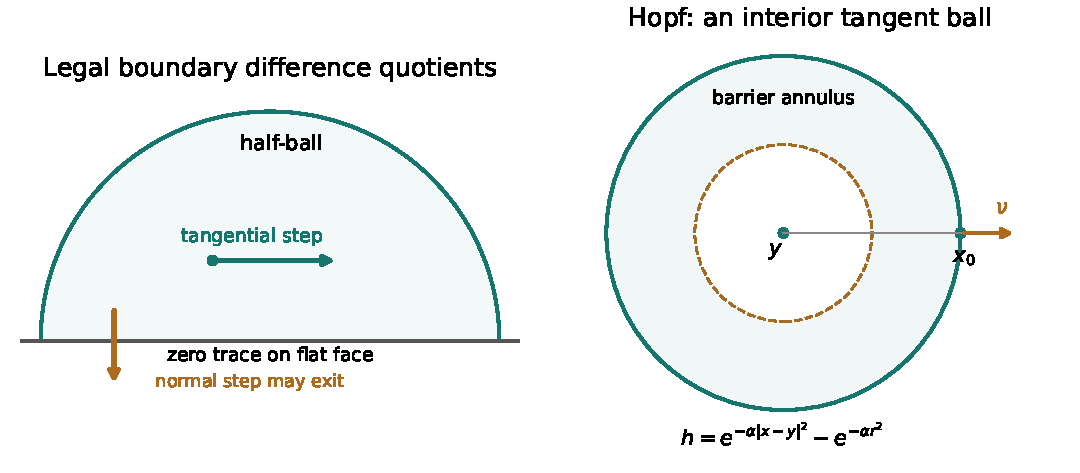
\includegraphics[width=\linewidth]{output/figures/ch06-boundary-tools.pdf}
\end{center}
{\small\textit{Two boundary mechanisms.} Tangential translations preserve
the flat zero-trace face; normal translations need not.
Hopf's exponential barrier is used only in the shaded annulus of an
interior tangent ball. Diagrams are schematic.}
\end{minipage}

\Needspace{35mm}
\subsection{Higher boundary regularity (Evans \S6.3.2, Theorems 5--6)}
\begin{theorem}\label{thm:6-higher-boundary}
If $\partial U$ is $C^{m+2}$, $A,b,c\in C^{m+1}(\overline U)$ and
$f\in H^m(U)$, then a weak zero-Dirichlet solution satisfies
\[
 u\in H^{m+2}(U),\qquad
 \|u\|_{H^{m+2}(U)}
 \leq C\bigl(\|f\|_{H^m(U)}+\|u\|_2\bigr).
\]
Smooth boundary, coefficients and data give $u\in C^\infty(\overline U)$.
\end{theorem}
\begin{expandedproof}
The case $m=0$ is Theorem~\ref{thm:6-boundary-h2}.
For the induction step assume $u\in H^{m+2}$ and $f\in H^{m+1}$,
with coefficients $C^{m+2}$ and boundary $C^{m+3}$.
In a flattened chart, differentiate $m+1$ times only tangentially.
The resulting derivative has zero trace on the flat face, because
tangential differentiation commutes with the trace at these orders.
Its localized equation has an $L^2$ right side: expand the commutators
exactly as in the interior proof. Cutoffs keep tests away from the
curved part of the chart. Applying boundary $H^2$ gives all derivatives
of total order $N=m+3$ having at most two normal differentiations.

Recover the others from \eqref{eq:6-normal-recovery}. To estimate an
order-$N$ derivative with $q\geq3$ normal indices, apply an order-$N-2$
derivative with $q-2$ normal indices to that identity.
The desired term is multiplied by $a^{nn}$; the other order-$N$ terms
have at most $q-1$ normal indices, and coefficient commutators contain
derivatives of $u$ of order at most $N-1$, already controlled.
Induct on $q$ and divide by $a^{nn}\geq\theta$.
These differentiated identities can be justified first by interior
regularity and then by the uniform estimates up to the flat face,
as in the $H^2$ case. Patching proves the global estimate.
Finally extend Sobolev functions across the smooth boundary and use
embedding at arbitrarily high orders to obtain $C^\infty(\overline U)$.
\end{expandedproof}
\Needspace{45mm}
\PDEAnnotation{边界光滑度不能省略}{内部正则性只看系数和右端，边界正则性还看区域形状。角点可能产生奇性；零边界条件本身并不能保证解在角点附近有平方可积的二阶导数。}
\paragraph{What the estimates actually say.}
The two-derivative gain is an a priori estimate for solutions, not an
existence theorem by itself. At an eigenvalue, the term $\|u\|_2$
cannot be removed: a nonzero eigenfunction solves a homogeneous
shifted equation. Nonzero boundary data require a sufficiently regular
lift before the zero-boundary theorem can be used.
% Evans 6.4: English printed p.323 / PDF p.340; Chinese printed p.229 / PDF p.247.
\Needspace{65mm}
\section{Maximum Principles}
\label{sec:6-4}
Here we use nondivergence notation
\[
 Lu=-a^{ij}u_{ij}+b^iu_i+cu.
\]
Assume $U$ bounded, $A$ uniformly elliptic, and coefficients bounded and
continuous unless a stronger hypothesis is stated.
Solutions are classical, $u\in C^2(U)\cap C(\overline U)$.
These are different assumptions from the measurable-coefficient weak theory.

\subsection{Weak maximum principles (Evans \S6.4.1, Theorems 1--2)}
\begin{theorem}\label{thm:6-weak-max}
If $c=0$ and $Lu\leq0$, then
$\max_{\overline U}u=\max_{\partial U}u$.
If $c\geq0$ and $Lu\leq0$, then
\[
 \max_{\overline U}u\leq\max_{\partial U}u^+.
\]
In particular, $Lu\leq Lv$ and $u\leq v$ on $\partial U$ imply $u\leq v$
in $U$ when $c\geq0$.
\end{theorem}
\Needspace{45mm}
\PDEAnnotation{先固定算子符号}{本章主部是负号 $-a^{ij}u_{ij}$。因此 $Lu\leq0$ 控制上界；在内部极大点，$Du=0$、$D^2u\leq0$，主部反而非负。换符号时不等式也要一起换。}
\begin{expandedproof}
First let $c=0$. A strict subsolution $Lu<0$ cannot have an interior
maximum: at such a point $Du=0$, $D^2u$ is negative semidefinite,
and $-A:D^2u\geq0$, a contradiction.
For a non-strict subsolution use $u_\varepsilon=u+\varepsilon e^{\tau x_1}$.
Since
\[
 L(e^{\tau x_1})=(-a^{11}\tau^2+b^1\tau)e^{\tau x_1}<0
\]
for a fixed sufficiently large $\tau$, $u_\varepsilon$ has its maximum
on the boundary. Let $\varepsilon\downarrow0$.

For $c\geq0$, on the open set $D=\{u>0\}$ the operator
$K=L-c$ satisfies $Ku=Lu-cu\leq0$.
Apply the zero-potential result on $D$; boundary values on
$\partial D\cap U$ are zero, while the remaining values come from
$\partial U$. The proof uses compact maxima and does not require a
smooth level-set boundary. If $D$ is empty the conclusion is immediate.
Apply this assertion to $u-v$ for comparison.
\end{expandedproof}
Applying the theorem to $-u$ gives the corresponding minimum principles.
The restriction on $c$ is substantive: on $(0,\pi)$,
$u=\sin x$ solves $-u''-u=0$ with zero boundary values but is positive inside.

\Needspace{45mm}
\PDEAnnotation{弱最大值原理中的“弱”}{这里“弱”表示结论只控制边界极值，并非指 Sobolev 弱解。对弱解也有相应原理，但必须说明测试函数和系数条件，不能混用两个含义。}
For comparison, a direct weak energy argument is available in divergence
form when $b\in C^1(\overline U)$ and
$c-\tfrac12\operatorname{div}b\geq0$.
For a weak subsolution with $u^+\in H^1_0(U)$, testing with $u^+$ gives
\[
 0\geq B[u,u^+]
 =\int A Du^+\cdot Du^+
  +\int(c-\tfrac12\operatorname{div}b)(u^+)^2
 \geq\theta\|Du^+\|_2^2.
\]
Thus $u\leq0$. The drift integral was integrated by parts after writing
$u^+Du^+=D((u^+)^2)/2$.
This sufficient energy condition is distinct from $c\geq0$ in the
classical nondivergence argument.

\Needspace{35mm}
\subsection{Hopf's boundary lemma (Evans \S6.4.2)}
\begin{lemma}\label{lem:6-hopf}
Suppose an interior ball $B_r(y)\subset U$ touches $\partial U$ at $x_0$,
$u(x)<u(x_0)=M$ for all $x\in U$, and $Lu\leq0$.
Assume either $c=0$, or $c\geq0$ and $M\geq0$.
If $u$ is $C^1$ at $x_0$ in the inward-ball neighborhood, then
\[
 \partial_\nu u(x_0)>0,\qquad \nu=(x_0-y)/r.
\]
At a smooth tangency this is the outward normal to $U$.
\end{lemma}
\begin{expandedproof}
On $r/2<|x-y|<r$, put
$h(x)=e^{-\alpha|x-y|^2}-e^{-\alpha r^2}$.
It is positive inside and zero on the outer sphere. A direct calculation,
with $s=|x-y|$, gives
\[
 Lh\leq e^{-\alpha s^2}
 \bigl(-4\theta\alpha^2s^2+
       2\alpha\operatorname{tr}A+2\alpha|b|s+c\bigr)\leq0
\]
for sufficiently large $\alpha$; for $c=0$ the same bound applies.
On the inner sphere $u-M$ has a strictly negative maximum, so choose
$\varepsilon>0$ with $u-M+\varepsilon h\leq0$ there.
It is also nonpositive on the outer sphere.
Moreover $L(u-M+\varepsilon h)\leq-cM\leq0$.
Comparison on the annulus gives $u-M\leq-\varepsilon h$.
Along the radius $x_0-t\nu$ divide by $t>0$ and let $t\downarrow0$:
\[
 \partial_\nu u(x_0)\geq-\varepsilon\partial_\nu h(x_0)
 =2\varepsilon\alpha r e^{-\alpha r^2}>0.
\]
\end{expandedproof}
\Needspace{45mm}
\PDEAnnotation{Hopf 引理提供严格斜率}{最大值原理只说内部不能超过边界。Hopf 引理进一步说：若内部严格更小，函数沿外法向到达边界极大值时必须有正斜率；内球条件保证可放入显式屏障。}

\Needspace{35mm}
\subsection{Strong maximum principle (Evans \S6.4.2, Theorems 3--4)}
\begin{theorem}\label{thm:6-strong-max}
Let $U$ be connected. If $Lu\leq0$ and $c=0$, attainment of a maximum
at an interior point forces $u$ to be constant.
For $c\geq0$ the same holds for a nonnegative interior maximum.
Dually, a nonpositive interior minimum of a supersolution forces constancy.
\end{theorem}
\begin{expandedproof}
Let $M=\max_Uu$, attained inside, and suppose both sets
$C=\{u=M\}$ and $V=\{u<M\}$ are nonempty.
A path inside $U$ from $V$ to $C$ shows that their common relative
boundary contains a point in $U$.
Choose $y\in V$ sufficiently close to this point so that the ball with
radius $\operatorname{dist}(y,C)$ is contained in $U$.
Its interior is in $V$ and its boundary touches $C$ at some $x_0\in U$.
Hopf's lemma on this ball gives a strictly positive radial derivative
at $x_0$. But $x_0$ is an interior maximum of a differentiable function,
so $Du(x_0)=0$. This contradiction proves the assertion.
The minimum statement follows by replacing $u$ by $-u$.
\end{expandedproof}
In particular, for $c\geq0$, a nonzero nonnegative supersolution
$Lu\geq0$ is strictly positive in a connected domain.

% Expanded special-case proof of Evans 6.4.3, Theorem 5.
\Needspace{35mm}
\subsection{Harnack's inequality (Evans \S6.4.3, Theorem 5)}
\begin{theorem}[Smooth principal-part case proved here]\label{thm:6-harnack}
Suppose $A$ is smooth and uniformly elliptic and
$-a^{ij}u_{ij}=0$, $u\geq0$ in $U$. For connected $V\Subset U$,
\[
 \sup_Vu\leq C\inf_Vu.
\]
The constant depends on the geometry of $V$ inside $U$, ellipticity and
local coefficient bounds, including the derivatives used below, but not on $u$.
\end{theorem}
\Needspace{45mm}
\PDEAnnotation{Harnack 是定量正性}{强最大值原理说非负非零解处处为正；Harnack 还控制内区任意两点的比值。它需要方程等式，不能随意用于只有单边不等式的函数。}
\begin{expandedproof}
\paragraph{1. Take a logarithm to estimate relative oscillation.}
First take $u>0$, and put $v=\log u$ and $w=a^{ij}v_iv_j$.
Then
\begin{equation}\label{eq:6-log}
 -a^{ij}v_{ij}=w,\qquad \theta|Dv|^2\leq w\leq\Lambda|Dv|^2.
\end{equation}
Interior smoothness justifies the following differentiations:
rewrite the smooth nondivergence equation in divergence form and
apply \S\ref{sec:6-3}. On a fixed compact region,
\[
 w_{kl}=2a^{ij}v_{ikl}v_j+2a^{ij}v_{ik}v_{jl}+R_{kl},
 \quad
 |R_{kl}|\leq\varepsilon|D^2v|^2+C_\varepsilon|Dv|^2.
\]
The remainder consists of $D^2A\,Dv\,Dv$ and $DA\,D^2v\,Dv$.
Differentiate \eqref{eq:6-log} once to obtain
$-a^{kl}v_{ikl}=w_i+(\partial_i a^{kl})v_{kl}$.
Also
$a^{ij}a^{kl}v_{ik}v_{jl}\geq\theta^2|D^2v|^2$;
this is seen by diagonalizing the positive matrix $A$ at the point.
Absorbing coefficient remainders gives, for
$\mathcal M=-a^{kl}\partial_{kl}-2a^{ij}v_j\partial_i$,
\[
 \mathcal Mw\leq-\gamma|D^2v|^2+C|Dv|^2
                \leq-\gamma_1w^2+Cw.
\]
The second inequality uses $w= -A:D^2v\leq C|D^2v|$.

\paragraph{2. Localize and retain the drift--cutoff error.}
Take $\zeta\in C^\infty_c(U)$ with $0\leq\zeta\leq1$ and $\zeta=1$
on a chosen ball $V$. Let $z=\zeta^4w$.
If its maximum is positive, it occurs where $\zeta>0$, and
$\zeta Dw=-4wD\zeta$. At this point $Dz=0$ and
$\mathcal Mz=-A:D^2z\geq0$.
Expanding the product yields
\[
 0\leq-\gamma_1\zeta^4w^2+
        C\zeta^2w+C\zeta^3w^{3/2}.
\]
The last term comes from
$-2ADv\cdot D(\zeta^4)\,w$ and uses $|Dv|\leq C\sqrt w$.
It must be included because this drift depends on $v$.
Set $Y=\zeta^2w$ at this maximum point. Then
\[
 \gamma_1Y^2\leq C(Y+Y^{3/2}).
\]
For $Y>0$, divide by $Y$ and solve the resulting quadratic inequality
in $\sqrt Y$ to get $Y\leq C$. Hence $z\leq C$ at its maximum,
and $w\leq C$, $|Dv|\leq C$ on $V$.

\Needspace{45mm}
\PDEAnnotation{对数变换后的漂移项}{新算子的漂移含有 $D\log u$，不能预先当成已有一致界的系数。截断计算保留三次项，再用四次项吸收，才能保证最终常数不依赖解。}
\paragraph{3. Integrate the logarithmic gradient.}
For $x,y$ in the ball, integrate along their segment:
$|v(x)-v(y)|\leq C|x-y|\leq C\operatorname{diam}V$.
Exponentiation bounds $u(x)/u(y)$.
For a general connected $V\Subset U$, cover it by finitely many balls
whose slightly larger concentric balls remain inside $U$.
A finite chain of overlapping balls connects their values; multiplying
the finitely many comparison constants proves the result.
Finally apply the estimate to $u+\delta$, which solves the same equation
because there are no lower-order terms, and let $\delta\downarrow0$.
\end{expandedproof}


\PDEBodyDiagram{6.4}{Local positivity comparisons propagate along a chain.}
{Choose overlapping balls whose slightly larger balls still lie inside $U$. Comparing at overlap points transfers a local Harnack bound from $x$ to $y$. The resulting constant depends on the finite chain and its distance from the boundary, which is why connected compact interior regions occur in the theorem.}
{ch06-harnack-chain}

\paragraph{Scope of the source theorem.}
Evans states Harnack for the full operator with lower-order terms
and indicates extensions to bounded measurable coefficients.
The proof supplied in the source, and reconstructed above, is restricted
to smooth $A$ and $b=c=0$. The broader theorem is a further regularity
result, cited there to Gilbarg--Trudinger; it is not proved by the
logarithmic computation above. In the general case $u+\delta$ need not
solve $Lu=0$, and differentiating measurable coefficients is unavailable.
% Evans 6.5: English printed p.333 / PDF p.350; Chinese printed p.236 / PDF p.254.
\Needspace{65mm}
\section{Eigenvalues and Eigenfunctions}
\label{sec:6-5}
Assume in this section that $U$ is bounded, connected and has smooth
boundary, and that all coefficients are smooth on $\overline U$.
This keeps the spectral arguments separate from technical boundary
regularity issues. Eigenfunctions have zero Dirichlet trace.

\subsection{Symmetric operators (Evans \S6.5.1, Theorem 1)}
First let $Lu=-\partial_j(a^{ij}u_i)$ with $A$ symmetric uniformly elliptic.
Then $B[u,v]=\int A Du\cdot Dv$ is a symmetric positive form.
\begin{theorem}\label{thm:6-symmetric-spectrum}
There are real eigenvalues, repeated according to multiplicity,
\[
 0<\lambda_1\leq\lambda_2\leq\cdots,\qquad\lambda_j\longrightarrow\infty,
\]
and a complete orthonormal basis $(w_j)$ of $L^2(U)$ such that
$Lw_j=\lambda_jw_j$. Each eigenspace is finite dimensional, and
$w_j\in C^\infty(\overline U)$.
\end{theorem}
\begin{expandedproof}
Let $S=L^{-1}:L^2\to L^2$. Lax--Milgram, Poincar\'e and Rellich show
that $S$ is bounded and compact. If $u=Sf$ and $v=Sg$, then
\[
 (Sf,g)=B[u,v]=(f,Sg),\qquad
 (Sf,f)=B[u,u]>0\quad(f\ne0).
\]
Thus $S$ is self-adjoint, positive definite, and injective.

For completeness we give the compact spectral argument.
Let $\mu_1=\sup_{\|f\|_2=1}(Sf,f)>0$.
For a maximizing sequence $f_k$, pass to a weakly convergent subsequence
$f_k\rightharpoonup f$ with $\|f\|_2\leq1$.
Compactness gives $Sf_k\to Sf$, so $(Sf,f)=\mu_1$.
If $\|f\|_2<1$, scaling $f$ to norm one increases this value, a
contradiction. First variation on the unit sphere gives $Sf=\mu_1 f$.

Its orthogonal complement is invariant under $S$, by self-adjointness.
Repeat the argument there, recording multiplicities, to obtain
$\mu_1\geq\mu_2\geq\cdots>0$ and orthonormal eigenvectors $w_j$.
There are infinitely many, since an injective operator on infinite
dimensional $L^2(U)$ cannot have finite-dimensional range.
Compactness forces $\mu_j\to0$: otherwise $(Sw_j)$ has pairwise distances
bounded below.
If the closed span of the $w_j$ had a nonzero orthogonal complement,
the restriction of $S$ to that complement would still be compact and
positive definite and hence would have a positive maximal eigenvalue.
That value would be at most every $\mu_j$, contradicting $\mu_j\to0$.
This proves completeness. Set $\lambda_j=\mu_j^{-1}$.
Finite multiplicity follows from compactness, and regularity bootstrapping
applied to $Lw_j=\lambda_jw_j$ gives smoothness.
\end{expandedproof}
\Needspace{45mm}
\PDEAnnotation{先研究紧的逆算子}{$L$ 在 $L^2$ 上是无界算子，不宜直接套紧算子的谱定理。其逆先提升到 $H^1_0$，再由紧嵌入回到 $L^2$；逆的特征值趋零，对应 $L$ 的特征值趋无穷。}

\Needspace{35mm}
\subsection{Rayleigh quotient and positivity (Evans \S6.5.1, Theorem 2)}

\Needspace{45mm}
\PDEAnnotation{能量空间中的归一化不同}{$w_j$ 在 $L^2$ 中长度为一，但能量长度是 $\sqrt{\lambda_j}$。因此能量空间的正交归一基是 $w_j/\sqrt{\lambda_j}$，这决定了能量展开中的权重。}
\begin{theorem}\label{thm:6-rayleigh}
The first eigenvalue satisfies
\[
 \lambda_1=\min_{\substack{u\in H^1_0(U)\\\|u\|_2=1}}B[u,u].
\]
A minimizer solves $Lu=\lambda_1u$. There is a strictly positive first
eigenfunction in $U$, and $\lambda_1$ is simple.
Every eigenfunction for a larger eigenvalue changes sign.
\end{theorem}
\begin{expandedproof}
The energy inner product is $B$, equivalent to the $H^1_0$ norm.
The functions $w_j/\sqrt{\lambda_j}$ are orthonormal for this inner product,
since $B[w_i,w_j]=\lambda_i(w_i,w_j)$.
They are complete in the energy space: if $B[u,w_j]=0$ for all $j$,
then $(u,w_j)=0$ for all $j$, hence $u=0$ by the $L^2$ basis.
Hilbert-space Parseval therefore gives
\begin{equation}\label{eq:6-energy-spectrum}
 B[u,u]=\sum_j\lambda_j|(u,w_j)|^2,\qquad
 \|u\|_2^2=\sum_j|(u,w_j)|^2 .
\end{equation}
The Rayleigh minimum follows, with equality at $w_1$.
Alternatively, the direct method gives a minimizer: bounded energy
gives weak $H^1_0$ convergence, Rellich preserves the $L^2$ normalization,
and weak lower semicontinuity preserves minimality.

Differentiating the quotient
$B[u+tv,u+tv]/\|u+tv\|_2^2$ at $t=0$ yields
$B[u,v]=\lambda_1(u,v)$ for every $v$.
If $u$ is a minimizer, $|u|\in H^1_0$ has the same norm and energy
by the Sobolev chain rule, so it is also a minimizer and hence smooth.
It satisfies $L|u|=\lambda_1|u|\geq0$.
The strong minimum principle, applied after rewriting $L$ in
nondivergence form with zero potential, shows $|u|>0$ in $U$.
Continuity and connectedness force $u$ to have one fixed sign.

If two first eigenfunctions were independent, take a linear combination
that vanishes at one interior point but is not identically zero.
It is again a first eigenfunction, contradicting the preceding strict
sign property. Thus the eigenspace is one dimensional.
An eigenfunction for $\lambda>\lambda_1$ is orthogonal to the positive
$w_1$, and consequently must take both signs.
\end{expandedproof}
\Needspace{45mm}
\PDEAnnotation{绝对值仍要通过变分方程}{不能直接对 $|u|$ 做经典二阶求导。先用 Sobolev 链式法则证明能量不变，因而它仍是极小元；再由 Euler 方程与正则性得到光滑性和严格正性。}
For $-\partial_{xx}$ on $(0,\ell)$,
$w_j=\sqrt{2/\ell}\sin(j\pi x/\ell)$ and
$\lambda_j=(j\pi/\ell)^2$. Their oscillations illustrate positivity
of the first mode and sign changes of the higher modes.


\par\noindent\begin{minipage}{\linewidth}
\begin{center}
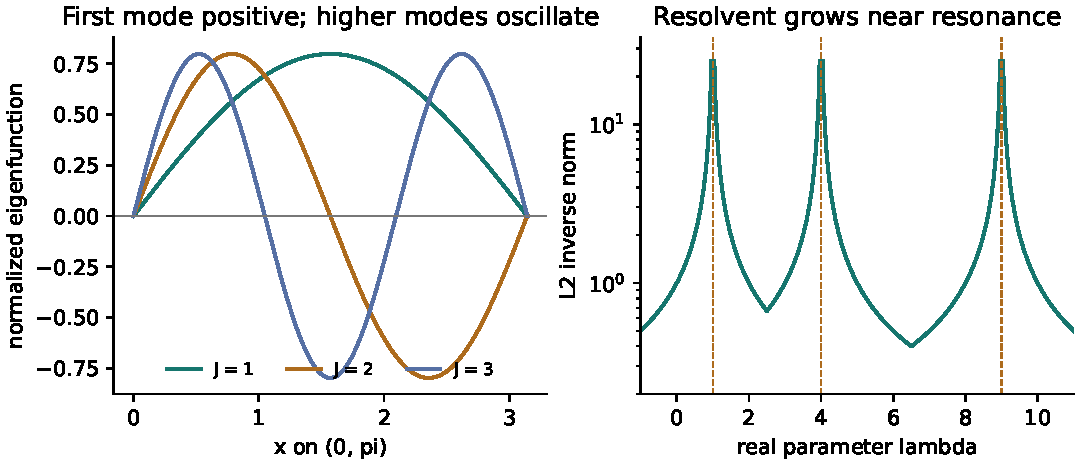
\includegraphics[width=\linewidth]{output/figures/ch06-modes-resonance.pdf}
\end{center}
{\small\textit{Explicit interval model.} On $(0,\pi)$ the Dirichlet
eigenvalues are $j^2$. For real $\lambda$ off the spectrum, the
self-adjoint inverse norm is
$\|(-\partial_{xx}-\lambda)^{-1}\|_{L^2\to L^2}
=1/\min_j|j^2-\lambda|$. The poles mark loss of uniqueness.}
\end{minipage}

\paragraph{Weyl's law: a source remark, not a proved theorem here.}
For the Dirichlet Laplacian on a smooth bounded domain,
\[
 N(\lambda):=\#\{j:\lambda_j\leq\lambda\}
 \sim \frac{\omega_n|U|}{(2\pi)^n}\lambda^{n/2}.
\]
Equivalently,
$\lambda_j\sim4\pi^2(j/(\omega_n|U|))^{2/n}$.
This asymptotic statement appears as a remark in Evans; its proof
requires additional spectral estimates and is not part of the
compactness argument above. Here $\omega_n$ is the volume of the unit ball.

% Expanded proof of Evans 6.5.2, Theorem 3; Schaefer is an external prerequisite.
\Needspace{35mm}
\subsection{A positive eigenfunction without symmetry (Evans \S6.5.2)}
Now write $L=-a^{ij}\partial_{ij}+b^i\partial_i+c$ and assume $c\geq0$.
The matrix $A$ is symmetric, but the full operator need not be self-adjoint.
For weak formulations and adjoints, first rewrite it in divergence form:
the drift in $B$ is $b^i+\partial_j a^{ij}$, rather than $b^i$ itself.

\begin{theorem}\label{thm:6-principal-nonsym}
There is a real eigenvalue $\lambda_1>0$ and an eigenfunction
$\phi>0$ in $U$, $\phi=0$ on $\partial U$.
Its eigenspace is one dimensional. Every complex eigenvalue $\lambda$
satisfies $\operatorname{Re}\lambda\geq\lambda_1$.
\end{theorem}
\Needspace{45mm}
\PDEAnnotation{非对称时换一种结构}{非对称算子通常没有正交特征基，Rayleigh 商也不再直接给出全部谱。主特征值的存在依赖紧逆算子保持非负性，极小实部则由正特征函数的商变换证明。}
\begin{expandedproof}
\paragraph{1. Construct a positive compact inverse.}
The homogeneous zero-Dirichlet problem has only the zero solution:
regularity makes a weak homogeneous solution classical, and comparison
applied to both signs gives zero. Fredholm therefore supplies $T=L^{-1}$.
Fix an integer $m>n/2+2$ and let $X=H^m(U)\cap H^1_0(U)$ with its $H^m$
norm. Boundary regularity makes $T:X\to H^{m+2}(U)\cap H^1_0(U)$ bounded,
so $T:X\to X$ is compact.
The closed convex cone $\mathcal C=\{u\in X:u\geq0\}$ is preserved by $T$.

Fix $0\ne w\in C^\infty_c(U)$, $w\geq0$.
The strong minimum principle and Hopf's lemma imply
$Tw>0$ inside and $\partial_\nu(Tw)<0$ on the boundary.
Since $w$ has compact support, some $\mu>0$ satisfies $\mu Tw\geq w$.

\paragraph{2. A compact fixed-point argument yields an eigenvector.}
We invoke the following \emph{external} form of Schaefer's theorem:
if a continuous compact map $F:\mathcal C\to\mathcal C$ has a bounded
set $\{u:u=tF(u),\ 0\leq t\leq1\}$, then $F$ has a fixed point.
This topological theorem is a prerequisite here, not proved in this chapter.

For $\varepsilon>0$, consider
\[
 u=\eta T(u+\varepsilon w),\qquad u\in\mathcal C.
\]
No solution can have $\eta>\mu$. Indeed positivity gives
$u\geq\varepsilon(\eta/\mu)w$; iterating $u\geq\eta Tu$ gives
$u\geq\varepsilon(\eta/\mu)^kw$ for every $k$, impossible at a point
where $w>0$.
If the solutions for $0\leq\eta\leq2\mu$ were bounded, Schaefer applied
to $F(u)=2\mu T(u+\varepsilon w)$ would give a solution at $\eta=2\mu$,
a contradiction. Hence that solution set is unbounded.
Choose $\varepsilon_j\downarrow0$ and solutions $u_j,\eta_j$ with
$\|u_j\|_X\geq\varepsilon_j^{-1}$ and $0\leq\eta_j\leq2\mu$.
Normalize $v_j=u_j/\|u_j\|_X$. Then
\[
 v_j=\eta_j T\left(v_j+\frac{\varepsilon_jw}{\|u_j\|_X}\right).
\]
Compactness gives a subsequence converging in $X$ to $v$ with
$\|v\|_X=1$, $v=\eta Tv$, and $\eta>0$ (otherwise the right side
would converge to zero). Thus $Lv=\eta v$, $v\geq0$.
Regularity, the strong minimum principle and Hopf give a smooth
$\phi=v>0$, $\partial_\nu\phi<0$, with $\lambda_1=\eta>0$.

\Needspace{45mm}
\PDEAnnotation{归一化保住非零极限}{紧性本身可能只给出零极限。把无界解列除以自身范数后，范数固定为一；扰动项同时趋零，极限才成为真正的非零特征函数。}
\paragraph{3. Exclude eigenvalues to the left of $\lambda_1$.}
For a complex eigenfunction $z$, smoothness and zero boundary values imply
$|z(x)|\leq C d(x)$ near the boundary, with
$d(x)=\operatorname{dist}(x,\partial U)$.
Hopf and compactness of $\partial U$ give $\phi(x)\geq a d(x)$.
For $0<\delta<1$, put $h=\phi^{1-\delta}$ and $v=z/h$.
Then $v$ extends continuously as zero on $\partial U$.

\PDEMarginDiagram{6.M}{商为何在边界趋零}
{由 $|z|\leq Cd$ 与 $\phi\geq ad$，得到 $|z|/\phi^{1-\delta}\leq C'd^\delta\to0$。图示上界取 $\delta=1/2$。}
{ch06-boundary-ratio-margin}

A product calculation gives
\[
 L(hv)=hKv+vLh,\qquad
 K=-A:D^2+(b-2AD\log h)\cdot D,
\]
and the chain rule gives
\[
 \frac{Lh}{h}
 =(1-\delta)\lambda_1+\delta c+
 \delta(1-\delta)\frac{A D\phi\cdot D\phi}{\phi^2}
 \geq(1-\delta)\lambda_1.
\]
Consequently, for $q=|v|^2$,
\[
 Kq=2\operatorname{Re}(\overline v Kv)-2A Dv\cdot D\overline v
 \leq2\left(\operatorname{Re}\lambda-\frac{Lh}{h}\right)q .
\]
If $\operatorname{Re}\lambda<\lambda_1$, choose $\delta$ small so that
the coefficient on the right is strictly negative.
The nonzero continuous function $q$, zero on $\partial U$, has a
positive interior maximum, where $Dq=0$ and $-A:D^2q\geq0$,
a contradiction. This argument is pointwise at that maximum; it does
not assume the drift $D\log h$ is bounded near the boundary.

\paragraph{4. Prove geometric simplicity by sliding positive functions.}
Let $z$ be a real eigenfunction for $\lambda_1$, changing its sign if
necessary so it is positive somewhere.
The estimates $\phi\geq a d$ and $|z|\leq C d$, also valid after adjusting
constants on the interior compact region, show that
\[
 t_*=\sup\{t\geq0:\phi-tz\geq0\text{ in }U\}
\]
is positive and finite. At $t_*$ the residual $r=\phi-t_*z$ is nonnegative
and satisfies $Lr=\lambda_1r\geq0$.
If it were nonzero, the strong minimum principle and Hopf would give
$r\geq a' d$. Since $|z|\leq C d$, a small further increase of $t_*$
would preserve nonnegativity, a contradiction.
Hence $r=0$. Apply this separately to real and imaginary parts for
complex eigenfunctions at the real value $\lambda_1$.
\end{expandedproof}

\Needspace{35mm}
\subsection{The positive adjoint eigenfunction}
\begin{lemma}\label{lem:6-positive-adjoint}
The formal Dirichlet adjoint has a positive eigenfunction $\phi^*$
for the same $\lambda_1$.
\end{lemma}
\begin{expandedproof}
The inverse $T^*$ is positive on $L^2$: for $f,g\geq0$,
$(T^*f,g)=(f,Tg)\geq0$.
Regularity makes its restriction to $X$ compact.
If $f\in\mathcal C$ is nonzero, $v=T^*f\geq0$ is nonzero.
Although the expanded potential $c^*$ of $L^*$ may be negative,
choose $M$ with $c^*+M\geq0$; then
$(L^*+M)v=f+Mv\geq0$.
The strong minimum principle and Hopf applied to $L^*+M$ give
$v>0$ and $\partial_\nu v<0$.
The compact-cone construction in Steps 1--2, with $T^*$ in place of $T$,
therefore gives $\phi^*>0$ and $L^*\phi^*=\lambda^*\phi^*$, $\lambda^*>0$.
Both eigenfunctions have zero trace, so weak adjointness yields
\[
 \lambda_1(\phi,\phi^*)=B[\phi,\phi^*]
 =(\phi,L^*\phi^*)=\lambda^*(\phi,\phi^*).
\]
The inner product is positive, hence $\lambda^*=\lambda_1$.
\end{expandedproof}
\Needspace{45mm}
\PDEAnnotation{伴随的零阶项可能变号}{原算子的 $c\geq0$ 不推出伴随算子的零阶项非负。先由逆算子的对偶关系得到非负性，再加常数使用强最大值原理，才能严谨得到伴随正特征函数。}
If $c$ has arbitrary sign but is bounded, apply the theorem to $L+\kappa$
with $c+\kappa\geq0$. Translating its eigenvalues back preserves the positive
principal eigenfunction, simplicity and the least-real-part property;
the resulting $\lambda_1$ need not be positive.
The word \emph{simple} above describes the eigenspace. In fact there is
also no generalized eigenvector at $\lambda_1$: an equation
$(L-\lambda_1)z=\phi$ contradicts pairing with $\phi^*$, since
$(\phi,\phi^*)>0$.

% Evans 6.6: English printed pp.343--348 / PDF pp.360--365.
\Needspace{65mm}
\section{Problems and Worked Solutions}
\label{sec:6-6}
These are concise restatements of the 17 source problems, with editorial
solutions. Unless a problem says otherwise, $U$ is bounded with smooth
boundary, coefficients are smooth and bounded, and ellipticity is uniform.
Connectedness is specified where constants or positivity are involved.
The same assumptions apply to each weak formulation below.

\Needspace{30mm}
\paragraph{1. Removing a potential by a positive solution.}
Relate $-\Delta u+cu=0$ to $-\operatorname{div}(aDv)=0$.
\begin{proof}[Solution]
If $w>0$ solves the first equation, set $u=wv$. The product rule gives
\[
 -\Delta(wv)+cwv
 =-w\Delta v-2Dw\cdot Dv+v(-\Delta w+cw)
 =-w^{-1}\operatorname{div}(w^2Dv).
\]
Thus $u$ solves the first equation exactly when $v=u/w$ solves the
second with $a=w^2$.
Conversely, given a smooth positive $a$, set $w=\sqrt a$ and
$c=\Delta w/w$. Then $-\Delta w+cw=0$, so the same identity proves
that $u=\sqrt a\,v$ solves the potential equation.
These are local identities wherever $w>0$; uniform bounds on $a$
are additional requirements for a uniform elliptic theory.
\end{proof}
\Needspace{45mm}
\PDEAnnotation{正解作为新的权重}{除以一个正解后，零阶项被吸收到权重 $w^2$ 中。关键是展开 $-\Delta(wv)$ 时保留两倍交叉项；反向构造的势是 $\Delta\sqrt a/\sqrt a$。}

\Needspace{30mm}

\Needspace{45mm}
\PDEAnnotation{负势可以由梯度能量吸收}{零阶系数略微为负并不立即破坏可解性。Poincar\'e 不等式把函数平方项转回梯度项；负势大小的阈值因此与区域几何有关。}
\paragraph{2. A small negative potential.}
For $L=-\partial_j(a^{ij}\partial_i)+c$, find $\mu>0$ so that
$c\geq-\mu$ ensures Lax--Milgram.
\begin{proof}[Solution]
Let $\|u\|_2\leq C_P\|Du\|_2$ on $H^1_0(U)$ and choose
$\mu=\theta/(2C_P^2)$. Then
\[
 B[u,u]\geq\theta\|Du\|_2^2-\mu\|u\|_2^2
 \geq\tfrac{\theta}{2}\|Du\|_2^2\geq C\|u\|_{H^1}^2.
\]
Bounded coefficients give boundedness of $B$. Apply
Theorem~\ref{thm:6-lax-milgram}. The permitted negative part depends on
both ellipticity and the domain's Poincar\'e constant.
\end{proof}

\Needspace{30mm}
\paragraph{3. The clamped biharmonic problem.}
For $f\in L^2(U)$, solve
$\Delta^2u=f$, with $u=\partial_\nu u=0$, weakly in $H^2_0(U)$.
\begin{proof}[Solution]
Use $B_2[u,v]=\int\Delta u\,\Delta v$ and $\ell(v)=\int fv$.
For $u\in C^\infty_c(U)$, integration by parts twice gives
\[
 \int(\Delta u)^2=\sum_{i,j}\int u_{ii}u_{jj}
                  =\sum_{i,j}\int u_{ij}^2.
\]
Approximation extends this to $H^2_0(U)$.
Since $u$ and each $u_i$ belong to $H^1_0(U)$, Poincar\'e applied twice
gives $\|u\|_{H^2}\leq C\|D^2u\|_2$.
Thus $B_2$ is bounded and coercive on $H^2_0$ and $\ell$ is bounded.
Lax--Milgram gives exactly one weak solution. On smooth boundaries
the closure definition of $H^2_0$ encodes both zero traces.
\end{proof}
\Needspace{45mm}
\PDEAnnotation{四阶方程用二阶能量空间}{双调和方程分部积分两次后只需二阶弱导数。$H^2_0$ 同时编码函数及一阶迹为零，不能用只有函数零迹的 $H^2\cap H^1_0$ 随意替代。}

\Needspace{30mm}
\paragraph{4. Neumann compatibility.}
For connected $U$, prove that
$\int Du\cdot Dv=\int fv$ for every $v\in H^1(U)$ is solvable exactly
when $\int_U f=0$.
\begin{proof}[Solution]
Testing with $v=1$ proves necessity. On
$V=\{u\in H^1(U):\int_Uu=0\}$, the mean-zero Poincar\'e inequality holds.
To see this, a counterexample can be normalized to have $\|u_j\|_2=1$,
mean zero and $\|Du_j\|_2\to0$.
Rellich gives a strong $L^2$ limit, whose weak gradient is zero.
It is constant by connectedness and zero by its mean, contradicting norm one.
Lax--Milgram on $V$ gives a unique mean-zero solution.
For arbitrary $v$, subtract its mean; the removed constant contributes
zero on both sides because $\int f=0$. Thus the full weak equation holds.
The difference of any two solutions has zero gradient, so all solutions
differ by a constant.
\end{proof}

\Needspace{30mm}
\paragraph{5. Robin boundary conditions.}
Formulate and solve $-\Delta u=f$, $u+\partial_\nu u=0$.
\begin{proof}[Solution]
Use $H^1(U)$ and its trace $T$, with
\[
 B_R[u,v]=\int_U Du\cdot Dv+\int_{\partial U}Tu\,Tv,\qquad
 \ell(v)=\int_Ufv.
\]
The plus boundary term follows from $\partial_\nu u=-u$ in Green's formula.
Trace boundedness makes $B_R$ bounded. Also
\[
 \|u\|_{H^1}^2\leq C\left(\|Du\|_2^2+
                            \|Tu\|_{L^2(\partial U)}^2\right).
\]
Otherwise normalize a violating sequence to norm one. Its gradients
and traces tend to zero; Rellich and weak $H^1$ convergence yield a
constant on each component, with zero trace, hence zero.
Strong $L^2$ convergence and vanishing gradients contradict norm one.
This proves coercivity; Lax--Milgram yields a unique solution for every $f$.
\end{proof}
\Needspace{45mm}
\PDEAnnotation{边界项也能控制常数}{Neumann 能量看不见常数，所以需要相容条件并允许加常数。Robin 能量多了边界平方项，常数方向也受到控制，于是无需零均值条件且解唯一。}

\Needspace{30mm}

\Needspace{45mm}
\PDEAnnotation{自然边界与本质边界}{Dirichlet 条件先限制解和测试函数所在空间，称为本质条件；Neumann 条件由分部积分后的边界项体现，称为自然条件。更换边界类型也就更换了变分空间。}
\paragraph{6. Mixed Dirichlet--Neumann data.}
Let connected $U$ have $\partial U=\Gamma_1\cup\Gamma_2$ with disjoint
closed pieces. Impose $u=0$ on $\Gamma_1$ and $\partial_\nu u=0$ on $\Gamma_2$.
\begin{proof}[Solution]
Set $V=\{u\in H^1(U):Tu=0\text{ on }\Gamma_1\}$ and require
$\int Du\cdot Dv=\int fv$ for every $v\in V$.
The Dirichlet condition is built into $V$; the Neumann condition appears
naturally after integration by parts.
If $\Gamma_1$ has positive surface measure, Poincar\'e holds on $V$:
a normalized counterexample converges to a constant by the argument
in Problem 4, and its zero trace on $\Gamma_1$ forces that constant to vanish.
Lax--Milgram gives existence and uniqueness for every $f$.
Under the stated smoothness and disjoint closed partition, a nonempty
$\Gamma_1$ is relatively open in $\partial U$ and has positive measure.
If $\Gamma_1$ is empty, Problem 4 gives the Neumann compatibility and
constant ambiguity. If $\Gamma_2$ is empty, this is the usual Dirichlet problem.
For more general partitions that meet along an interface, the weak
formulation still makes sense, but global $H^2$ regularity is a separate issue.
\end{proof}

\Needspace{30mm}
\paragraph{7. A monotone semilinear estimate.}
Let $u\in H^1(\R^n)$ have compact support and solve
$-\Delta u+c(u)=f$ weakly, where $c$ is smooth, $c(0)=0$, $c'\geq0$,
and $c(u),f\in L^2(\R^n)$. Prove $\|D^2u\|_2\leq C\|f\|_2$.
\begin{proof}[Solution]
For fixed $h$ in direction $e_k$, use
$v=-\delta_{-h}\delta_hu\in H^1(\R^n)$, an admissible compactly
supported weak test by density.
Discrete integration by parts gives
\[
 \|\delta_hDu\|_2^2+
 \int_{\R^n}\delta_h(c(u))\,\delta_hu
 =-\int_{\R^n}f\,\delta_{-h}\delta_hu.
\]
The second term is nonnegative because
$(c(s)-c(t))(s-t)\geq0$. Moreover,
$\|\delta_{-h}\delta_hu\|_2\leq\|\partial_k\delta_hu\|_2
\leq\|\delta_hDu\|_2$.
Hence $\|\delta_hDu\|_2\leq\|f\|_2$ uniformly in $h$.
The difference quotient criterion in each direction yields $u\in H^2$ and,
for the Frobenius norm, $\|D^2u\|_2\leq\sqrt n\,\|f\|_2$.
No upper bound on $c'$ is required in this monotonicity argument.
\end{proof}
\Needspace{45mm}
\PDEAnnotation{单调性替代导数上界}{非线性项的差商乘积非负，因此可以留在左边后直接舍去。这里使用的是 $c$ 的单调性，不需要把 $c'(u)$ 当作有界系数来估计。}

\Needspace{30mm}
\paragraph{8. Bernstein's gradient estimate.}
For $Lu=-a^{ij}u_{ij}=0$, show that
$v=|Du|^2+Mu^2$ is a subsolution for large $M$ and deduce a boundary estimate.
\begin{proof}[Solution]
Differentiate the equation to get
$Lu_k=(\partial_k a^{ij})u_{ij}$. Thus
\[
 L|Du|^2
 =-2a^{ij}u_{ki}u_{kj}
       +2u_k(\partial_k a^{ij})u_{ij}
 \leq-\theta|D^2u|^2+C|Du|^2 .
\]
Also $L(u^2)=-2a^{ij}u_i u_j\leq-2\theta|Du|^2$.
Choose $2M\theta\geq C$. Then $Lv\leq0$.
The weak maximum principle gives
$\sup_U|Du|^2\leq\sup_{\partial U}(|Du|^2+Mu^2)$, hence
\[
 \|Du\|_{L^\infty(U)}
 \leq C\bigl(\|Du\|_{L^\infty(\partial U)}
               +\|u\|_{L^\infty(\partial U)}\bigr).
\]
\end{proof}

\Needspace{30mm}
\paragraph{9. A boundary barrier estimate.}
For $Lu=-a^{ij}u_{ij}=f$, $u=0$ on $\partial U$, suppose
$Lw\geq1$, $w\geq0$ on $\partial U$, and $w(x_0)=0$.
\begin{proof}[Solution]
The minimum principle gives $w\geq0$ in $U$.
Let $F=\|f\|_\infty$. Since
$L(\pm u-Fw)\leq0$ and $\pm u-Fw\leq0$ on the boundary,
comparison gives $|u|\leq Fw$.
Assuming the indicated boundary derivatives exist, evaluate at
$x_0-t\nu$ and divide by $t$ to obtain
$|\partial_\nu u(x_0)|\leq F|\partial_\nu w(x_0)|$.
All tangential derivatives of the smooth zero-boundary function $u$
vanish at $x_0$, so $|Du(x_0)|=|\partial_\nu u(x_0)|$.
This is the desired estimate, with constant $F$.
\end{proof}
\Needspace{45mm}
\PDEAnnotation{屏障把函数值变成法向斜率}{先比较得到整个区域的 $|u|\leq\|f\|_\infty w$，再沿内法线取差商。边界上 $u$ 恒为零，所以梯度只剩法向分量。}

\Needspace{30mm}

\Needspace{80mm}
\PDEAnnotation{同一唯一性可有两种证明}{能量法用积分把整个梯度消掉；最大值原理通过极值位置与边界斜率制造矛盾。前者更适合弱解，后者直接揭示正性与边界几何的作用。}
\paragraph{10. Harmonic Neumann solutions are constant.}
Give energy and maximum-principle proofs on connected $U$.
\begin{proof}[Solution]
Green's identity gives
$\int_U|Du|^2=-\int_Uu\Delta u+\int_{\partial U}u\partial_\nu u=0$,
so $Du=0$ and connectedness gives constancy.
Alternatively, if $u$ were nonconstant, its maximum would be on the
boundary by the strong maximum principle and all interior values would
be strictly smaller. Hopf's lemma at a boundary maximum would imply
$\partial_\nu u>0$, contradicting the homogeneous Neumann condition.
The latter proof uses a smooth boundary, or at least the needed interior ball.
\end{proof}

\Needspace{30mm}
\paragraph{11. Convex functions of weak solutions.}
If bounded $u\in H^1(U)$ satisfies
$\int A Du\cdot Dv=0$ for $v\in H^1_0(U)$, prove that
$w=\varphi(u)$ is a weak subsolution for smooth convex $\varphi$.
\begin{proof}[Solution]
The bounded range of $u$ makes $\varphi',\varphi''$ bounded on that range,
so $w\in H^1(U)$ and $Dw=\varphi'(u)Du$.
First take bounded $0\leq v\in H^1_0(U)$.
The product $\varphi'(u)v\in H^1_0(U)$ is an admissible test and gives
\[
 \int A Dw\cdot Dv
 =-\int \varphi''(u)v\, A Du\cdot Du\leq0 .
\]
For arbitrary $0\leq v\in H^1_0(U)$, use
$v_M=\min(v,M)$ and pass in the left side by $v_M\to v$ in $H^1$.
This proves the required inequality for every nonnegative weak test.
The function $w$ need not have zero trace.
\end{proof}
\Needspace{45mm}
\PDEAnnotation{测试函数的乘积要先检查}{若 $v$ 无界，$\varphi''(u)vDu$ 未必属于 $L^2$，不能直接宣布 $\varphi'(u)v$ 合法。先截断 $v$，证明不等式后再用 $H^1$ 收敛去掉截断。}

\Needspace{30mm}
\paragraph{12. A positive supersolution implies comparison.}
Assume $h\in C^2(U)\cap C(\overline U)$,
$h>0$ on \emph{all of} $\overline U$, and $Lh\geq0$.
Prove the zero-boundary weak maximum principle without assuming $c\geq0$.
\begin{proof}[Solution]
For $Lu\leq0$ and $u\leq0$ on $\partial U$, set $z=u/h$.
The product formula gives
\[
 Lu=hMz+zLh,\qquad
 M=-A:D^2+(b-2ADh/h)\cdot D.
\]
On $\{z>0\}$, $Mz\leq0$ and $M$ has no potential.
For each $\varepsilon>0$, the closure of $\{z>\varepsilon\}$ is compact
in $U$, because $z\leq0$ on the boundary and $\min_{\overline U}h>0$.
The drift is bounded there, so the zero-potential maximum principle
gives $z\leq\varepsilon$ on this set, which must therefore be empty.
Let $\varepsilon\downarrow0$.
Positivity only in $U$ would not suffice:
$h=\sin x$ for $L=-\partial_{xx}-1$ on $(0,\pi)$ is an interior
positive solution but vanishes at the endpoints, and comparison fails.
\end{proof}

\Needspace{30mm}
\paragraph{13. Courant's max--min principle.}
For the symmetric operator of \S\ref{sec:6-5}, show
\[
 \lambda_k=\max_{\dim S=k-1}\ \min_{\substack{u\in H^1_0(U)\cap S^\perp\\\|u\|_2=1}} B[u,u],
\]
where $S\subset H^1_0(U)$ and orthogonality is in $L^2(U)$.
\begin{proof}[Solution]
For any such $S$, linear algebra supplies a nonzero vector in
$\operatorname{span}(w_1,\ldots,w_k)\cap S^\perp$.
Normalize it. Formula~\eqref{eq:6-energy-spectrum} gives its energy
at most $\lambda_k$, so the inner minimum is at most $\lambda_k$.
For $S=\operatorname{span}(w_1,\ldots,w_{k-1})$, every admissible $u$
has only modes $j\geq k$, and the same formula gives
$B[u,u]\geq\lambda_k$. Equality occurs at $w_k$.
For any fixed $S$, the minimum exists by the direct method; its
orthogonality constraints are preserved by strong $L^2$ convergence.
\end{proof}
\Needspace{45mm}
\PDEAnnotation{极小极大中的正交空间}{这里去掉的是前若干模态在 $L^2$ 中的方向。任意少于 $k$ 个线性约束都不可能消灭前 $k$ 个模态的全部组合，这就是一半不等式的有限维理由。}

\Needspace{30mm}

\Needspace{45mm}
\PDEAnnotation{非对称公式中的权重来自伴随}{不能只对 $Lu/u$ 做普通空间平均。与正的伴随特征函数配对后，正确权重是 $u\phi^*$；分部积分才把这个加权平均固定为主特征值。}
\paragraph{14. A principal-eigenvalue max--min formula.}
For the nonsymmetric operator, prove
\[
 \lambda_1=\sup_{\substack{u\in C^\infty(\overline U),\
                  u>0\text{ in }U\\u=0\text{ on }\partial U}}
                  \ \inf_{x\in U}\frac{Lu(x)}{u(x)}.
\]
\begin{proof}[Solution]
Let $\phi^*>0$ be the adjoint eigenfunction from
Lemma~\ref{lem:6-positive-adjoint}. Both functions have zero trace,
so Green's identity, or the weak adjoint identity, gives
\[
 \int_U\phi^*Lu=\int_UuL^*\phi^*
                =\lambda_1\int_Uu\phi^*.
\]
Thus the weighted average of $Lu/u$ with positive weight $u\phi^*$
is $\lambda_1$. Its infimum cannot exceed this average.
If the infimum is $-\infty$ the inequality is immediate; otherwise
integrating its pointwise lower bound proves it directly.
Taking $u=\phi$ achieves equality everywhere.
A constant shift handles potentials of arbitrary bounded sign.
\end{proof}

\Needspace{30mm}
\paragraph{15. Hadamard's domain-variation formula.}
Let $-\Delta w=\lambda w$ on a smoothly moving domain $U(\tau)$,
$w=0$ on its boundary and $\int_{U(\tau)}w^2=1$.
Assume a smooth eigenvalue/eigenfunction branch, and denote boundary
velocity by $\mathbf v$.
\begin{proof}[Solution]
Use the Eulerian derivative $\dot w$ at a fixed spatial point.
Differentiating $w(x(\tau),\tau)=0$ on the moving boundary gives
\[
 \dot w=-Dw\cdot\mathbf v
       =-\partial_\nu w\,(\mathbf v\cdot\nu).
\]
Reynolds' formula for normalization yields
$2\int_Uw\dot w+\int_{\partial U}w^2\mathbf v\cdot\nu=0$,
hence $\int_Uw\dot w=0$.
Since $\lambda=\int_U|Dw|^2$, differentiate once more:
\begin{align*}
 \dot\lambda
 &=2\int_U Dw\cdot D\dot w+
             \int_{\partial U}|Dw|^2\mathbf v\cdot\nu\\
 &=2\lambda\int_Uw\dot w+
      2\int_{\partial U}\partial_\nu w\,\dot w+
             \int_{\partial U}(\partial_\nu w)^2\mathbf v\cdot\nu\\
 &=-\int_{\partial U}(\partial_\nu w)^2\mathbf v\cdot\nu.
\end{align*}
Tangential derivatives vanish because $w$ is zero on the boundary.
The smooth-branch hypothesis is essential; a multiple eigenvalue need
not admit a single arbitrarily chosen differentiable eigenfunction branch.
\end{proof}
\Needspace{45mm}
\PDEAnnotation{扩张区域使特征值下降}{若边界向外移动，$\mathbf v\cdot\nu>0$，公式给出 $\dot\lambda<0$。负号来自移动边界条件 $\dot w=-\partial_\nu w\,\mathbf v\cdot\nu$，不是凭直觉添加。}

\Needspace{30mm}

\Needspace{45mm}
\PDEAnnotation{辐射条件选择向外传播}{时间因子取 $e^{-i\sigma t}$ 时，$e^{i\sigma r}/r$ 描述向外传播的球面波。条件中的减号与这一时间约定配套；平面波不会在所有方向都向外辐射。}
\paragraph{16. Helmholtz waves and radiation.}
Let real $\sigma\ne0$ and $\lambda=\sigma^2$.
\begin{proof}[Solution]
(a) For $|\omega|=1$,
$-\Delta e^{i\sigma\omega\cdot x}=\sigma^2e^{i\sigma\omega\cdot x}$.
Thus $e^{i\sigma(\omega\cdot x-t)}$ solves the wave equation.

(b) In dimension three put
$\Phi(x)=e^{i\sigma r}/(4\pi r)$, $r=|x|$.
The radial identity $\Delta g=g''+2g'/r$ shows
$(-\Delta-\sigma^2)\Phi=0$ for $r>0$.
At $r=\varepsilon$,
\[
 -\int_{\partial B_\varepsilon}\partial_r\Phi\,dS
 =e^{i\sigma\varepsilon}(1-i\sigma\varepsilon)\longrightarrow1.
\]
Integration by parts against a smooth test function outside
$B_\varepsilon$ therefore gives
$(-\Delta-\sigma^2)\Phi=\delta_0$; the other shrinking-sphere term and
the volume integral of $\sigma^2\Phi$ tend to zero.

(c) For $\Phi$,
$r(\Phi_r-i\sigma\Phi)=-e^{i\sigma r}/(4\pi r)\to0$ uniformly in angle.
For the plane wave at $x=r\vartheta$,
\[
 r(w_r-i\sigma w)
 =i\sigma r(\omega\cdot\vartheta-1)e^{i\sigma r\omega\cdot\vartheta},
\]
whose modulus diverges on every ray with $\omega\cdot\vartheta\ne1$.
Thus the plane wave does not satisfy the Sommerfeld condition.
\end{proof}

\Needspace{30mm}
\paragraph{17. Uniqueness of an entire radiating solution.}
Suppose $w$ solves $-\Delta w=\sigma^2w$ throughout $\R^3$ and satisfies
$r(w_r-i\sigma w)\to0$ \emph{uniformly in angle}. Prove $w=0$.
\begin{proof}[Solution]
Green's identity and the real coefficient $\sigma^2$ imply
\[
 0=\int_{\partial B_R}(\overline w\,w_r-w\,\overline{w_r})\,dS.
\]
The imaginary flux is zero, so expansion of the square gives
\[
 \int_{\partial B_R}(|w_r|^2+\sigma^2|w|^2)\,dS
 =\int_{\partial B_R}|w_r-i\sigma w|^2\,dS=o(1).
\]
Uniform radiation justifies the last step, since the sphere has area
$4\pi R^2$ and the integrand is $o(R^{-2})$ uniformly.
For a fixed $x_0$ and $R>|x_0|$, Green's representation with the
outgoing kernel $\Phi(x-x_0)$ gives
\[
 w(x_0)=\int_{\partial B_R}
   \bigl(\Phi\,w_r-w\,\partial_r\Phi\bigr)\,dS .
\]
Here $\partial_r$ on the kernel means the outward derivative on
$\partial B_R$, not radial differentiation about $x_0$.
For large $R$, both $\Phi(x-x_0)$ and this derivative are $O(R^{-1})$,
so their $L^2(\partial B_R)$ norms remain bounded.
Cauchy--Schwarz and the vanishing flux norm above imply $w(x_0)=0$.
Since $x_0$ was arbitrary, $w\equiv0$.
\end{proof}
\Needspace{45mm}
\PDEAnnotation{辐射条件还包含一致性}{从逐方向极限跳到球面积分极限需要控制角变量。这里明确采用对方向一致的 Sommerfeld 条件；基本解在原点有奇性，所以并不违背“全空间光滑辐射解只能为零”。}

% Evans 6.7: English printed p.348 / PDF p.365; Chinese printed p.246 / PDF p.264.
\Needspace{65mm}
\section{References and Proof Dependencies}
\label{sec:6-7}
The primary source is Lawrence C. Evans, \emph{Partial Differential
Equations}, second edition, Chapter~6, printed pp.~293--348
(local English PDF pp.~310--365). The Chinese scan corresponds to
printed pp.~208--246 (PDF pp.~226--264); selected page comparisons
are recorded in \texttt{docs/CHAPTER-06.md}.
The English prose, proof expansions, solutions and Chinese annotations
here are editorial reconstructions.

Evans's references point to Gilbarg--Trudinger for weak elliptic theory,
regularity, maximum principles and Harnack; Krylov and
Ladyzhenskaya--Uraltseva for regularity; Protter--Weinberger and
Pucci--Serrin for maximum principles; and Smoller for spectral theory.
For domain variations the source cites Garabedian; for radiation it
cites Colton. These are source bibliography pointers, not claims
that those books have been independently consulted for this draft.

\paragraph{Dependencies and boundaries.}
Riesz representation, Hilbert weak compactness and Hilbert Parseval
are prerequisites. Chapter~5 supplies the Sobolev tools.
Lax--Milgram, the compact Fredholm lemma, regularity, maximum principles,
the smooth principal-part Harnack inequality, compact self-adjoint
spectral decomposition and the principal-eigenvalue arguments are
expanded above. The nonsymmetric existence proof explicitly invokes
Schaefer's fixed-point theorem. Weyl's law is stated as an unproved
source remark. The general measurable-coefficient Harnack theorem
is described as an extension, not claimed as proved.
All 17 source problems have editorial solutions.
Compilation, model calculations and layout checks do not constitute
independent mathematical review; this chapter remains an author-checked
study draft.